\section{Einführung}\label{sec:einfuehrung}
Der folgende Bericht gibt einen Überblick über den Entwurf und die Umsetzung einer solarbetriebenen Wetterstation im Rahmen der Sensortechnikvorlesung. Hierbei sollen zunächst die Anforderungen und bereits vorhandene Konzepte/Komponenten kurz vorgestellt und dann sowohl auf die Soft- als auch die Hardwareseitige Umsetzung eingegangen werden.

\subsection{Die Wetterstation}\label{subsec:Wetterstation}
\begin{figure}[H]
  \centering
  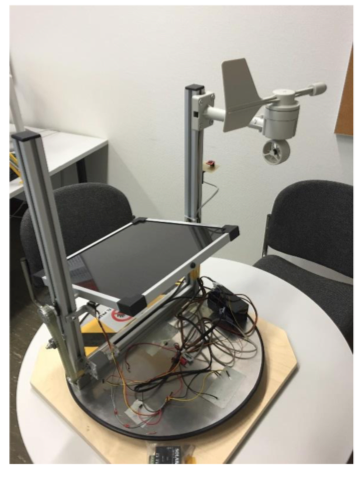
\includegraphics[width=0.5\textwidth]{./img/Wetterstation.png}
  \caption{Gegebener Aufbau der Wetterstation}\label{fig.wetterstation}
\end{figure}

In Abbildung \ref{fig.wetterstation} ist der gegebene Aufbau der Wetterstation dargestellt. Dieser besteht aus einem kippbaren Solarpanel, das auf einer drehbaren Platte montiert ist. Sowohl Dreh- als auch Kippbewegung wird über jeweils einen Getriebemotor ermöglicht. Des Weiteren ist bereits eine Windfahne zur Erfassung der Windrichtung und -geschwindigkeit montiert.

\subsection{Anforderungen}\label{subsec:Anforderungen}
Die Wetterstation soll folgende Werte erfassen:

\begin{itemize}
\item Temperatur
\item Luftdruck
\item Luftfeuchte
\item Höhe über NN
\item Windgeschwindigkeit
\item Windrichtung
\item Standort
\end{itemize}

Weiterhin soll die Wetterstation über das Solarpanel mit Strom versorgt werden, wobei aber dieses durch einen 12V Akku gepuffert werden soll, um z.B. die Nachtstunden ohne Ausfall der Spannungsversorgung überbrücken zu können. Für eine optimale Energieausbeute soll das Panel abhängig vom Sonnenstand über die beiden Getriebemotoren ausgerichtet werden. Außerdem soll der Akkuzustand erfasst und die drahtlose Kommunikation mit einem PC ermöglicht werden. Schließlich sollen die erfassten Sensordaten auf einer SD-Karte gespeichert werden.


\subsection{Vorüberlegungen}\label{subsec:Vorueberlegungen}
Bevor die beschriebenen Anforderungen umgesetzt werden, sind einige Vorüberlegungen und die Auswahl der geeigneten Sensorik nötig. Letztere werden ausführlich in Abschnitt \ref{sec:Sensoren} dargestellt. Die Drahtloskommunikation soll über ein Bluetooth-Modul realisiert und um eine eigene GUI, die die Darstellung aktueller Sensordaten auf einem PC ermöglicht, erweitert werden. Des Weiteren wird die bisher vorhandene Windfahne ausgetauscht und ersetzt, da diese nur über eine unzureichende Dokumentation verfügt.
Ebenfalls ist eine wasserdichte Ausführung der Wetterstation wünschenswert, die Umsetzbarkeit muss überprüft werden. Um Energie zu sparen, soll die Ausrichtung der Wetterstation sowie die Abfrage der Sensordaten nicht kontinuierlich sondern in noch festzulegenden Zeitabständen erfolgen.
%%% Local Variables:
%%% mode: latex
%%% TeX-master: "../termpaper"
%%% End:
